\documentclass[12pt]{article}

\usepackage[a4paper,left=25mm,right=10mm,top=20mm,bottom=20mm]{geometry}
\usepackage{setspace}
\onehalfspacing
\usepackage{times}
\usepackage[T2A]{fontenc}
\usepackage[utf8]{inputenc}
\usepackage[russian,english]{babel}
\usepackage{graphicx}
\usepackage{float}
\usepackage{hyperref}

\graphicspath{{figures/}}

\begin{document}

\begin{titlepage}
\begin{center}
\textbf{NATIONAL RESEARCH UNIVERSITY}\\
\textbf{HIGHER SCHOOL OF ECONOMICS}\\[1.2cm]
Faculty of Computer Science\\
Bachelor's Programme ``Data Science and Business Analytics''\\[2.2cm]
\textbf{Research Project Report on the Topic:}\\[0.4cm]
\textbf{Research on Fairness and Bias in Machine Learning Models for HR Automation}\\[3.0cm]
\end{center}

\noindent
\begin{minipage}[t]{0.58\textwidth}
Fulfilled by:\\
Student of the Group 233\\
Aleko Maisuradze
\end{minipage}%
\begin{minipage}[t]{0.42\textwidth}
\centering
13.01\\[-0.4em]
\rule{0.9\linewidth}{0.4pt}
\end{minipage}

\vfill
\begin{center}
Moscow, 2026
\end{center}
\end{titlepage}

\selectlanguage{english}
\tableofcontents
\newpage

\selectlanguage{russian}
\section*{Аннотация}
Проект посвящён исследованию fairness и bias в моделях машинного обучения для HR-автоматизации. Основная цель состоит в том, чтобы проверить, проявляются ли демографические различия в HR-данных и в предсказаниях моделей, а также оценить, насколько методы bias mitigation уменьшают fairness gaps и какой ценой для predictive performance. Репозиторий проекта содержит код, исходные данные, визуализации и таблицы, позволяющие проверить каждое численное утверждение из отчёта.

\selectlanguage{english}
\section*{Abstract}
This project investigates fairness and algorithmic bias in machine learning models used for HR automation. The study focuses on measurable demographic disparities in HR attrition prediction, the behavior of fairness metrics across groups, and the trade-off between bias mitigation and predictive performance. The accompanying repository is organized so that report claims can be traced to executable code and generated CSV artifacts.

\section*{Keywords}
fairness, algorithmic bias, HR automation, employee attrition, demographic parity, equalized odds

\newpage

\section{Introduction}
Machine learning systems are increasingly used in human resource management for employee attrition prediction, candidate screening, performance analytics and workforce planning. These systems promise more efficient and standardized decision-making, but they also create fairness risks because HR decisions directly affect people's careers, income stability and professional opportunities.

Algorithmic bias can appear even when protected attributes are removed from the dataset. Historical HR data may reflect unequal organizational structures, and variables such as income, job level, overtime and tenure can act as proxies for demographic attributes. Therefore, fairness in HR automation cannot be reduced to removing columns such as Gender or Age. It requires systematic evaluation of outcomes, predictions and model errors across groups.

The research question is: do HR-related machine learning models show measurable demographic disparities, and can bias mitigation methods reduce these disparities without unacceptable loss of predictive performance? This question is answered through pre-registered hypotheses, baseline models, fairness metrics, mitigation experiments and bootstrap confidence intervals.

\section{Literature Review}
Barocas and Selbst (2016) show that data-driven systems may create disparate impact through proxies and historical bias. Kleinberg et al. (2017) demonstrate that several fairness criteria cannot generally be satisfied simultaneously when base rates differ across groups. Hardt et al. (2016) introduce equality of opportunity and equalized odds as practical group fairness criteria. Raghavan et al. (2020) discuss practical barriers in algorithmic hiring systems. These works motivate the empirical evaluation framework used in this project.

\section{Methodology}
\subsection{Data}
The empirical analysis uses the IBM HR Employee Attrition dataset. The target variable is Attrition, converted to a binary variable. The protected attributes used in the first stage are Gender and AgeGroup. Age is grouped as $<30$, $30$--$40$ (employees in their thirties) and $40+$.

\subsection{Hypotheses}
H1 states that removing protected attributes will not eliminate fairness gaps completely because proxy variables remain in the data. H2 states that age-related fairness gaps will be larger than gender-related gaps. H3 states that reweighting will reduce demographic parity gap but may reduce predictive performance. H4 states that tree-based models will improve ROC-AUC but not necessarily fairness.

\subsection{Exploratory Data Analysis}
\begin{figure}[H]
\centering
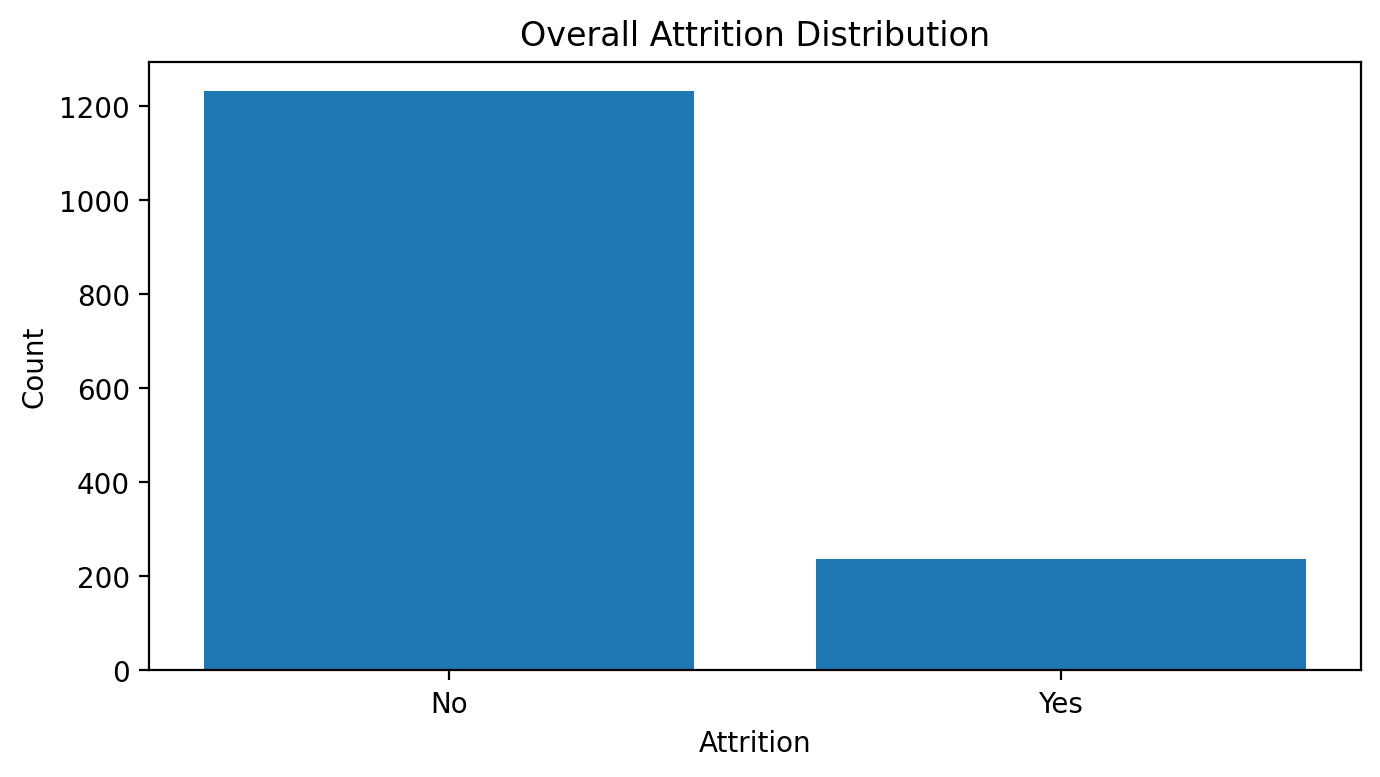
\includegraphics[width=0.85\textwidth]{fig_attrition_distribution.png}
\caption{Overall attrition distribution. The dataset is imbalanced, which motivates using metrics beyond accuracy.}
\end{figure}

\begin{figure}[H]
\centering
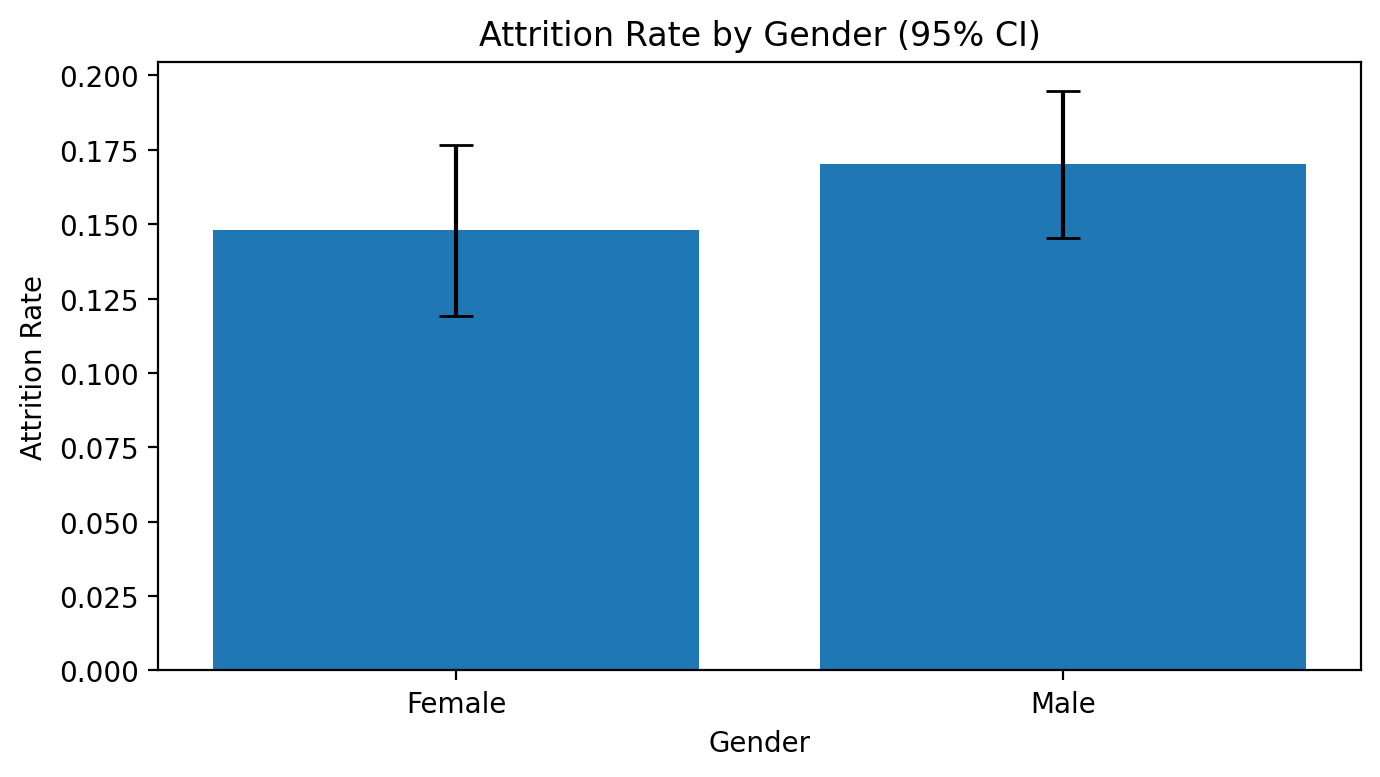
\includegraphics[width=0.85\textwidth]{fig_attrition_by_gender_ci.png}
\caption{Attrition rate by gender with 95 percent confidence intervals. This figure checks whether the raw outcome differs across gender groups.}
\end{figure}

\begin{figure}[H]
\centering
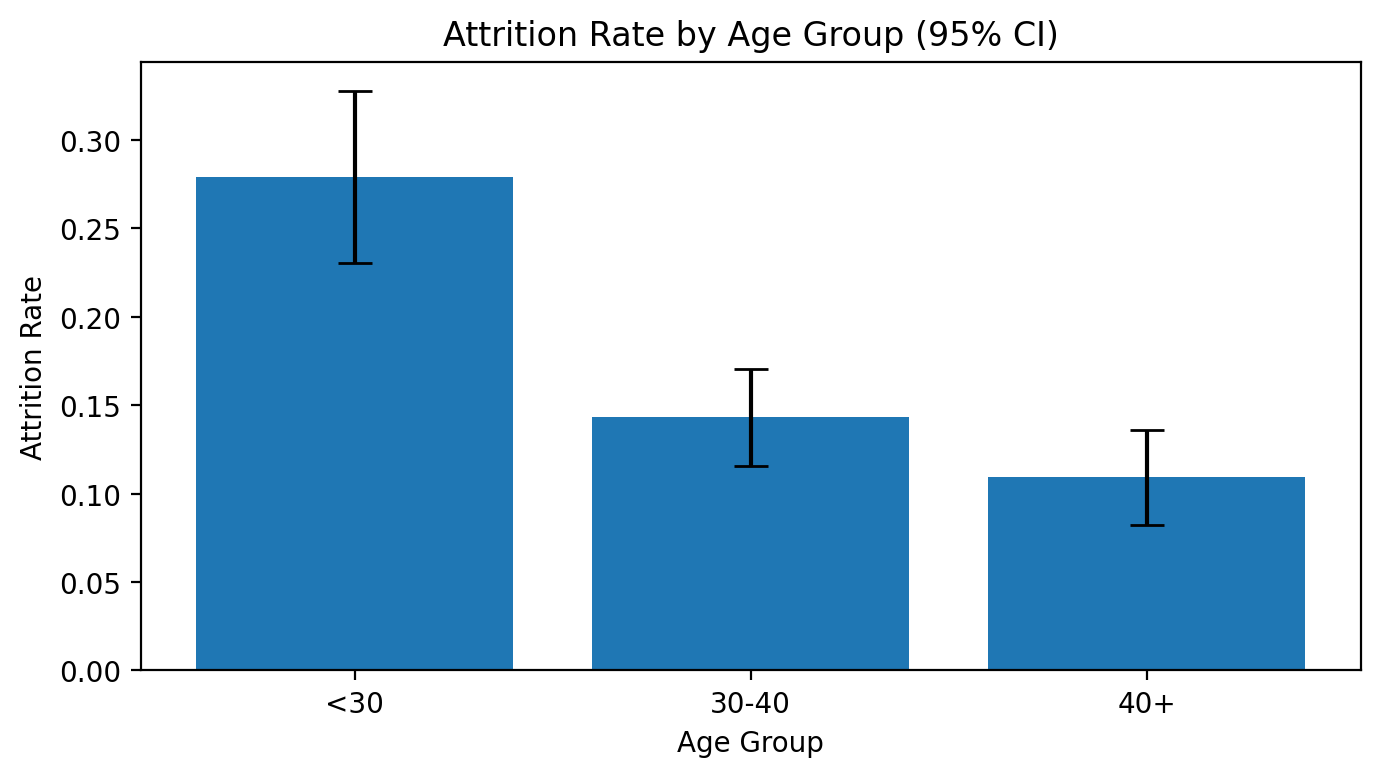
\includegraphics[width=0.85\textwidth]{fig_attrition_by_agegroup_ci.png}
\caption{Attrition rate by age group with 95 percent confidence intervals. The youngest group has visibly higher attrition rate.}
\end{figure}

\begin{figure}[H]
\centering
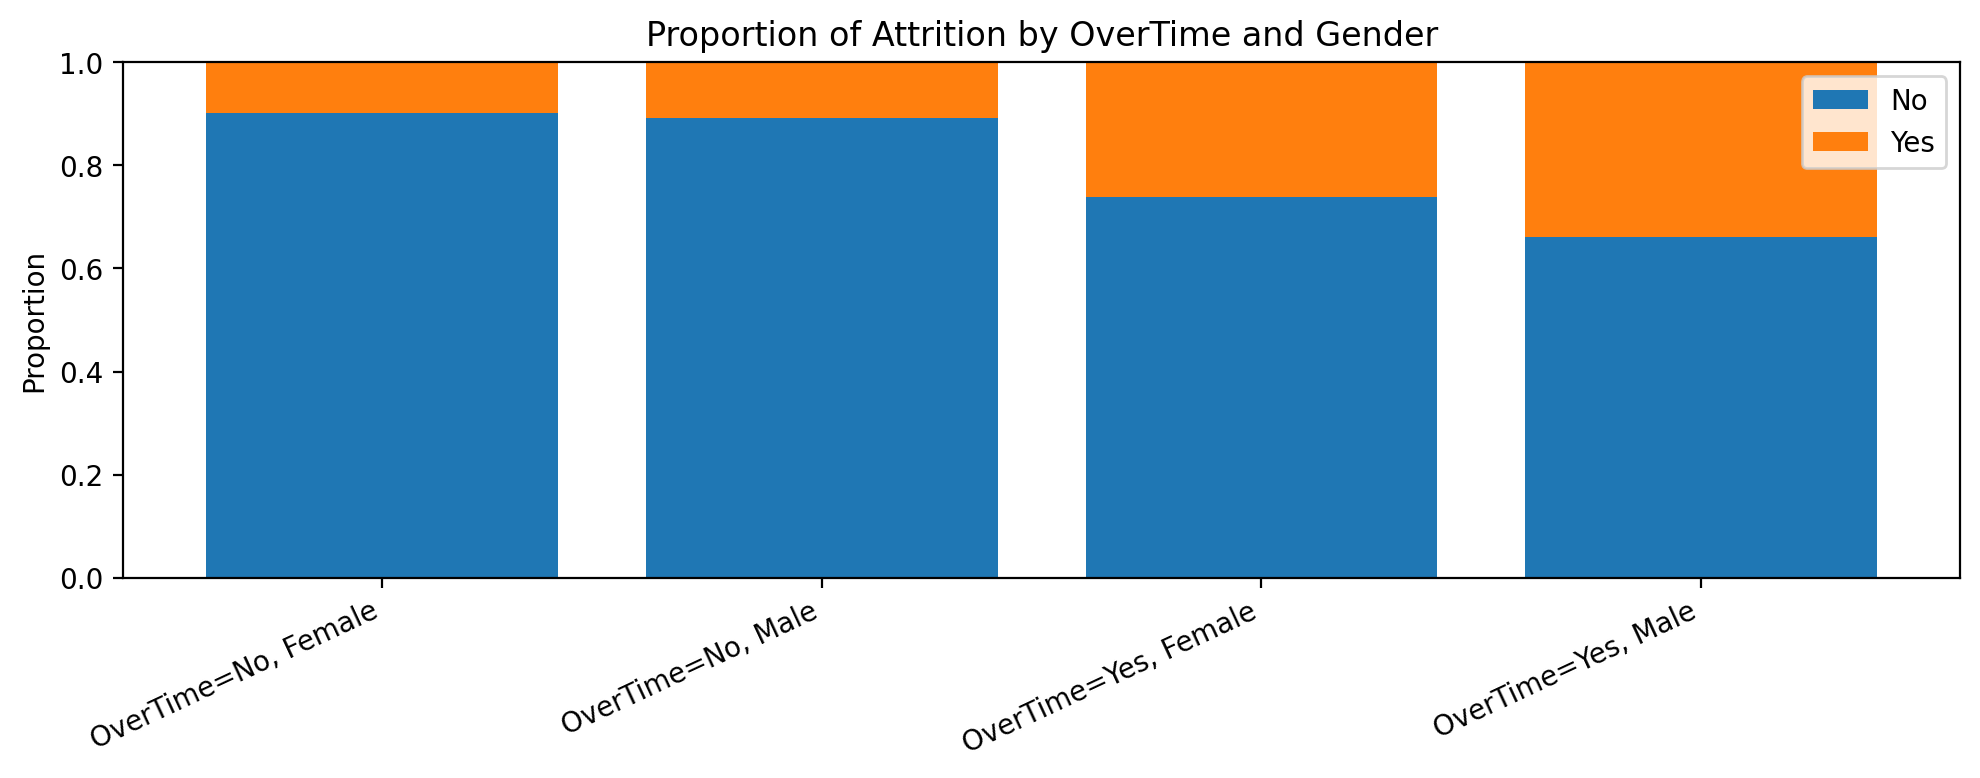
\includegraphics[width=0.95\textwidth]{fig_attrition_overtime_gender.png}
\caption{Attrition proportion by overtime and gender. This figure checks interaction effects that may become proxy pathways.}
\end{figure}

\begin{figure}[H]
\centering
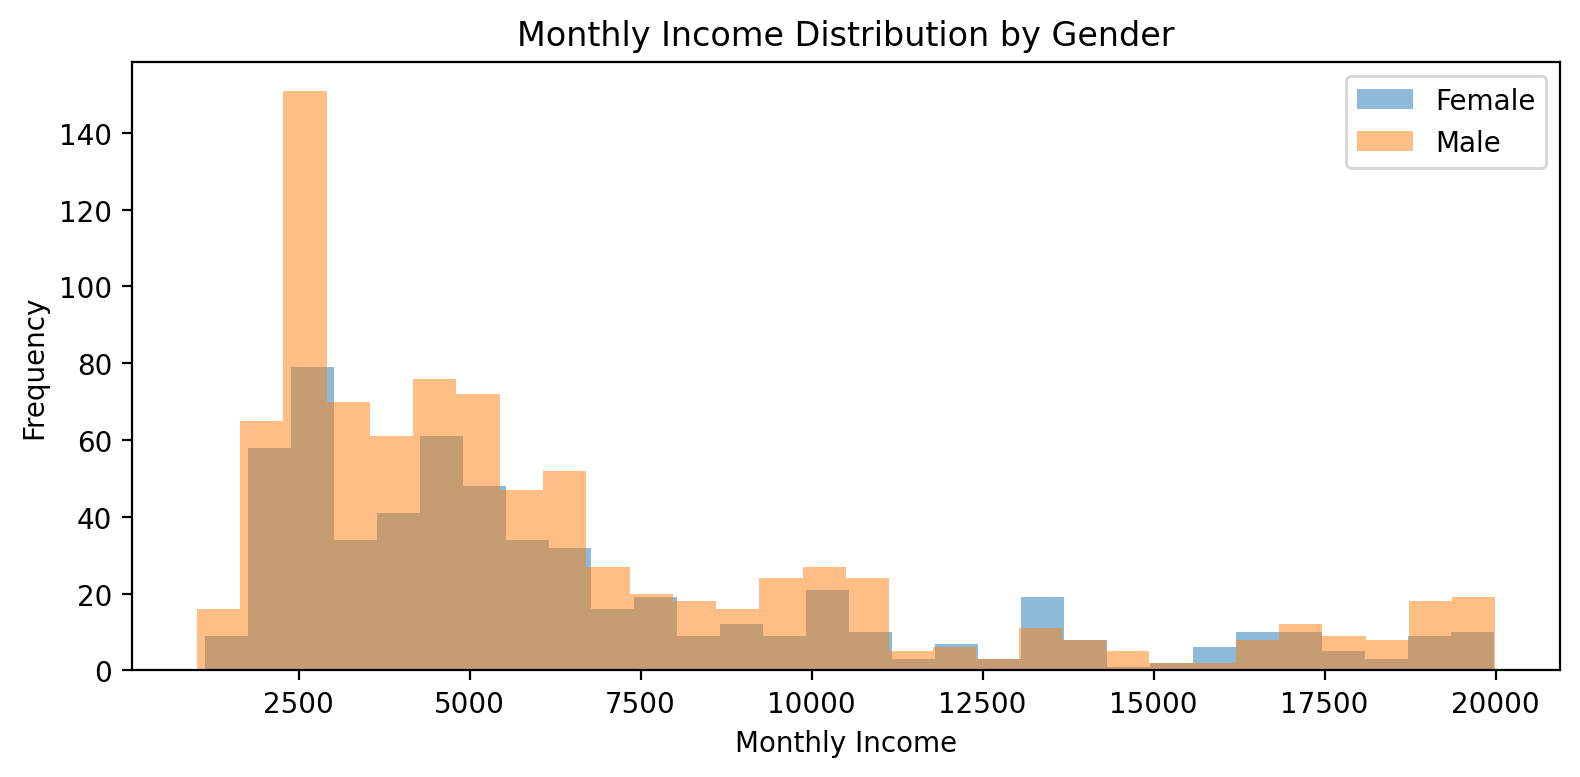
\includegraphics[width=0.90\textwidth]{fig_income_distribution_by_gender.png}
\caption{Monthly income distribution by gender. Income-related variables may partially encode demographic information.}
\end{figure}

\begin{figure}[H]
\centering
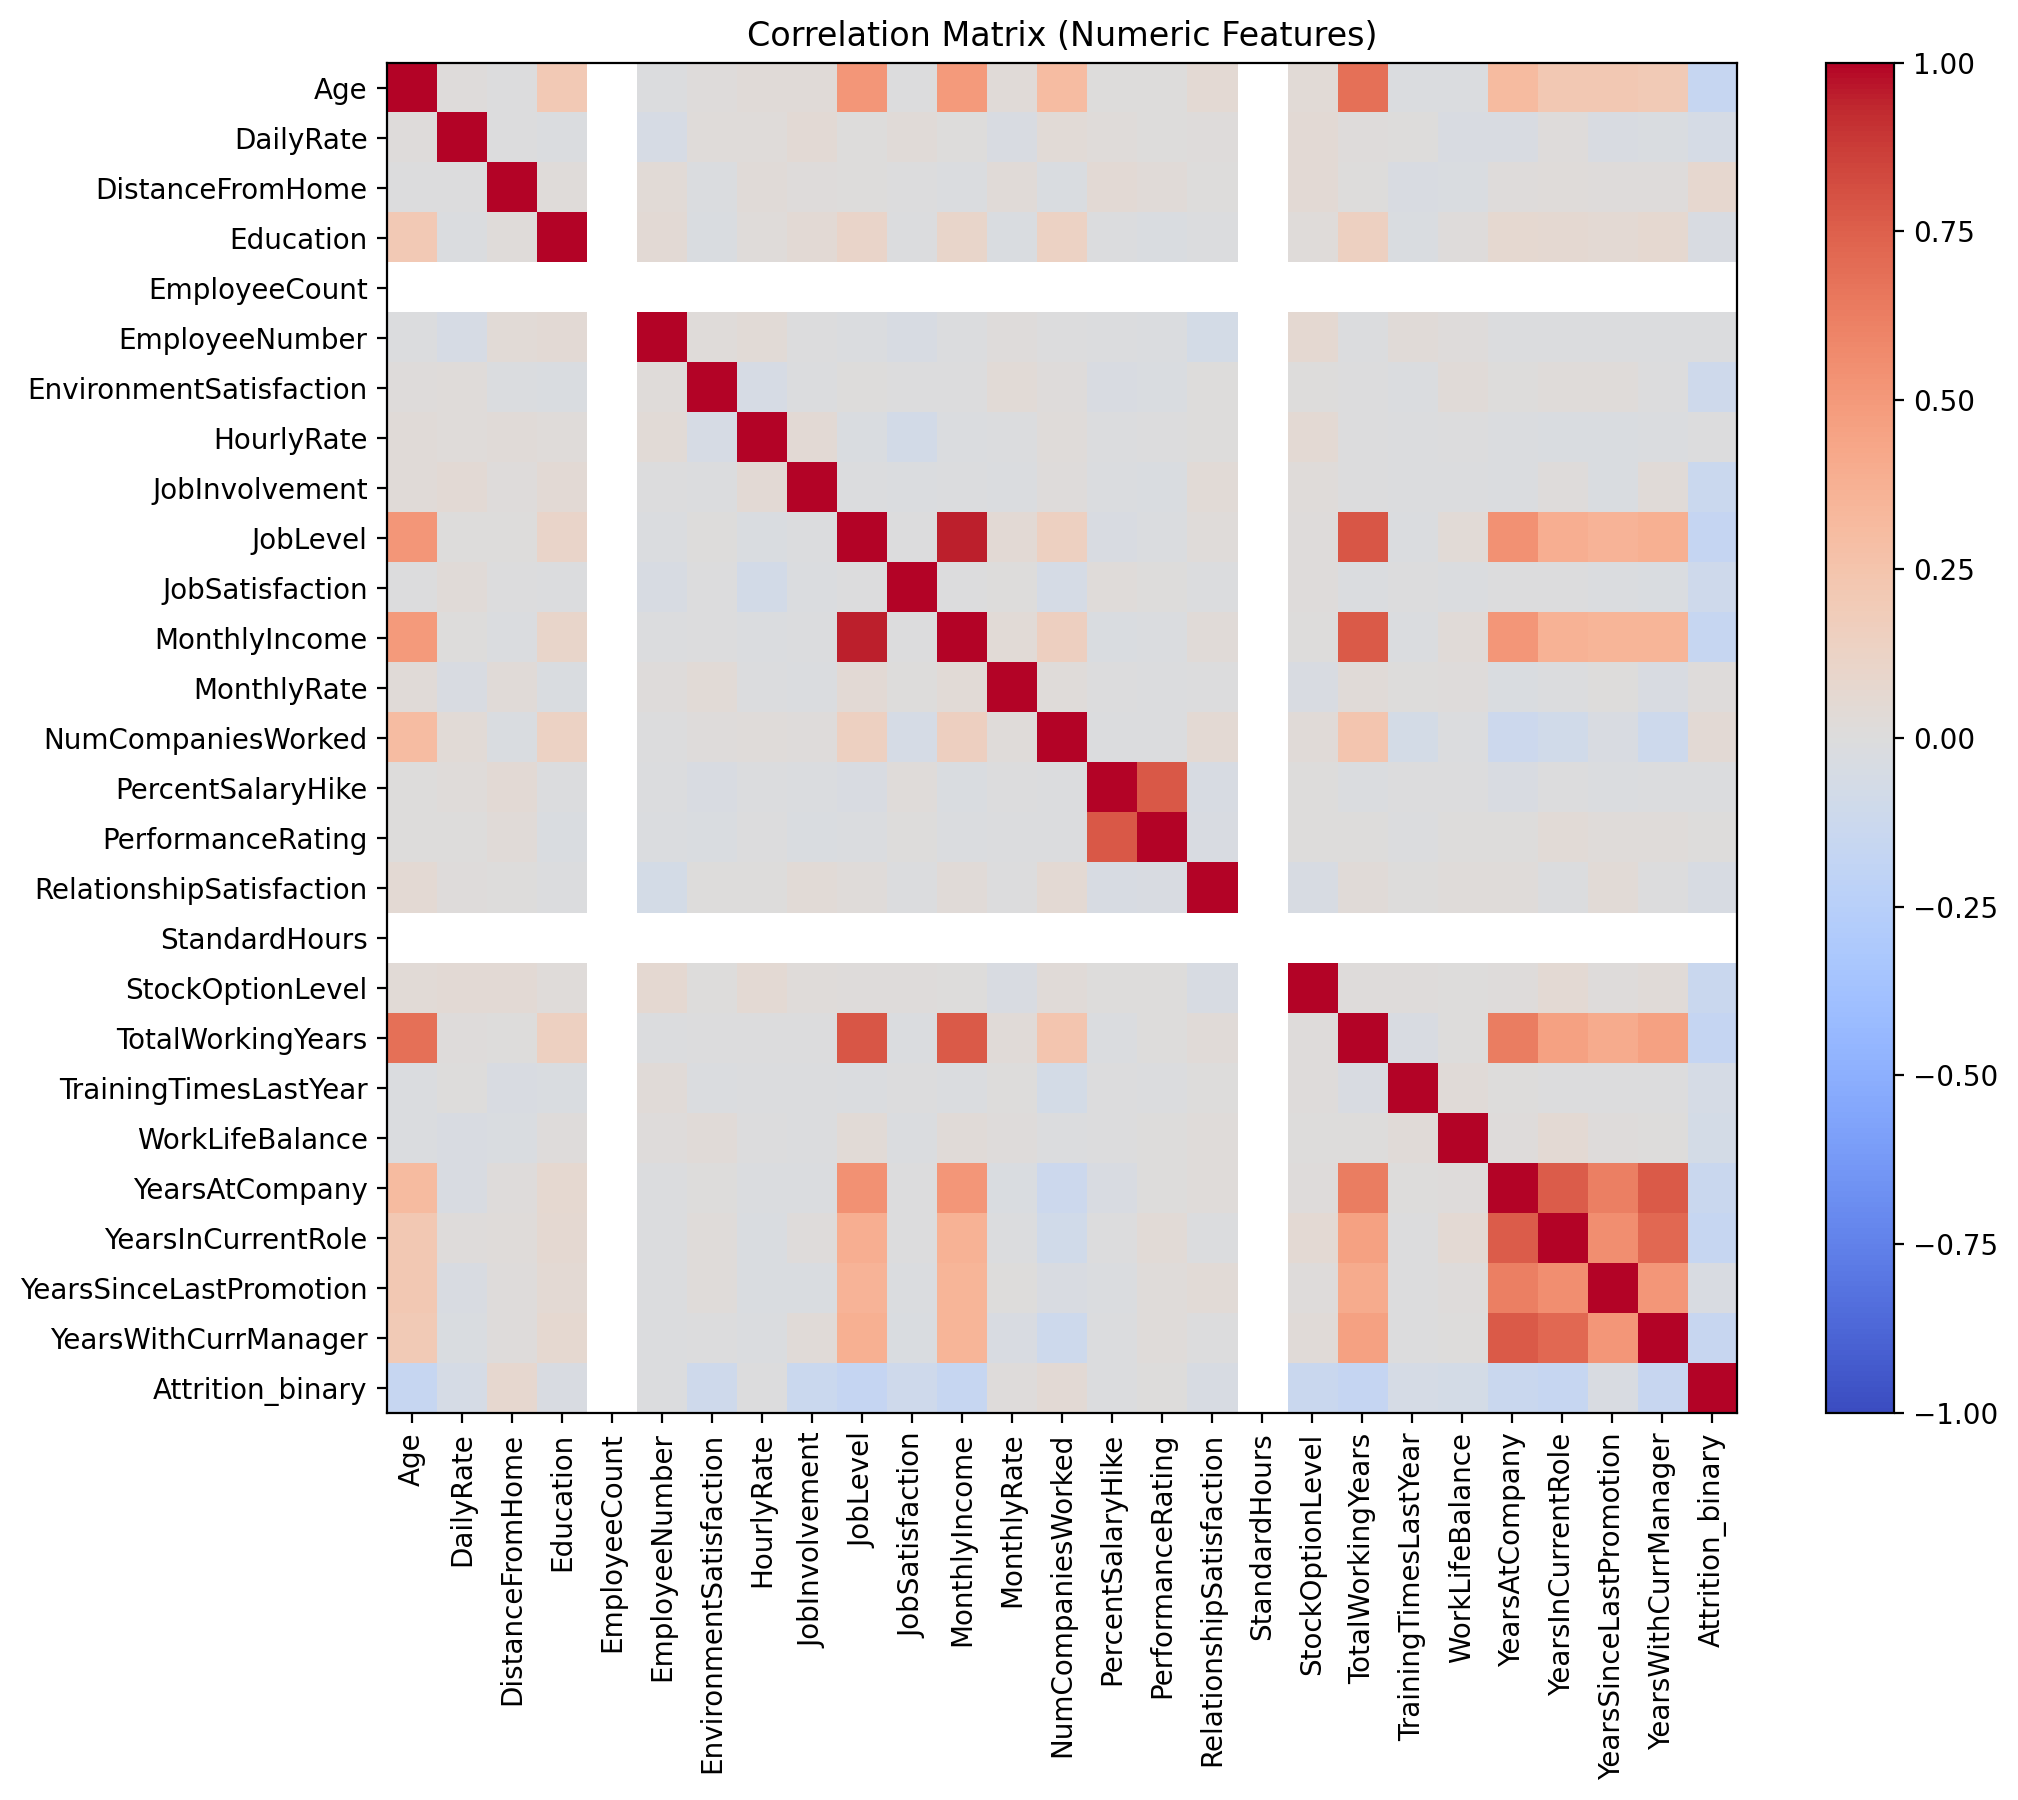
\includegraphics[width=0.98\textwidth]{fig_correlation_matrix_numeric.png}
\caption{Correlation matrix for numeric features. Strong correlations between income, job level and experience variables indicate possible proxy effects.}
\end{figure}

\subsection{Models and Metrics}
The baseline models are Majority Class, Logistic Regression with all features, Logistic Regression without protected attributes, Random Forest and Gradient Boosting. Performance is evaluated by accuracy, F1-score and ROC-AUC. Fairness is evaluated by demographic parity gap, equality of opportunity gap and equalized odds gap for Gender and AgeGroup.

\subsection{Reproducibility and Claim Traceability}
The repository generates CSV files in \texttt{outputs/} and rounded report tables in \texttt{reports/tables/}. The file \texttt{outputs/claims\_traceability.csv} maps report-style claims to the exact generated artifact and filter used to support them. This structure makes statements such as ``this group has a higher metric by this amount'' directly checkable from code.

\subsection{Statistical Validation}
Bootstrap confidence intervals are computed for the main Logistic Regression baseline. The final notebook and generated tables report each hypothesis as supported, not supported, partially supported or inconclusive based on the pre-defined thresholds.

\section{Limitations}
The IBM HR dataset is limited in size and does not contain race. Therefore, the main analysis focuses on Gender and AgeGroup. The dataset is also a public benchmark, so conclusions should be interpreted as a controlled case study rather than direct evidence about a specific real employer.

\section{Future Work}
Future work will extend the analysis to additional HR datasets, include more mitigation methods and compare model behavior under more realistic deployment scenarios.

\section{Conclusion}
This project provides a reproducible framework for evaluating fairness and bias in HR machine learning systems. The repository links report claims to executable code, figures, metrics and hypothesis-level conclusions.

\end{document}
